% !Mode:: "TeX:UTF-8"

\chapter{文献综述}{Literature Review}
\label{chap02}

长期以来,众多经济学家和金融学家对\ts 的形成机制投入了大量的精力与心血。对\ts 的研究经历了从传统的以解释其形成机理为主的定性分析到以统计拟合与预测为主的现代定量分析的发展过程,产生了大量的用于解释\ts 的形成机制与动态特征的\tsm{}。 本章将对相关文献进行梳理,对现代利率期限结构模型研究的文献资料进行回顾及评述。这部分将着重介绍\dns 的发展过程及其后的拓展模型,探讨\ts 动态行为可分解为具有平稳特征的长期均衡状态下的利率均值回复部分与非平稳的时变部分,并指出长期均衡利率水平的平稳组成部分由具有稳定可预测性的\dsf 决定,从而在现有模型的基础上引入\dsf 的分析。

\section{利率期限结构:理论与模型}{Term Structure Theory and Modeling}

\subsection{基本概念介绍}
在深入探讨本文所论述的研究问题之前,我们首先来给出一些在金融经济理论与债券市场分析中常用的基本概念,并由此来介绍一些本文使用的数学符号与标记。

\subsubsection{银行账户}

银行账户(Bank Account),也称做货币市场账户,指的是市场投资者将资金投放在一个具有较低风险性质、同时具有较高流动性功能的短期账户。我们用$B(t)$来表示该账户随时间变化的动态轨迹,则
\begin{align}
\mbox{连续时间\qquad} dB(t) &= r_t B(t) dt, \label{bank-account}\\
\mbox{离散时间\qquad}  B(t + \Delta t) &= B(t) (1 + r_t \Delta t), 
\end{align}
其中,$r_t$为短期利率水平。相对离散时间模型而言,连续时间模型在数学建模上更为复杂,但它能够提供充分的特性来得到更精确的理论解和更精练的经验假设。鉴于篇幅所限,本文将主要讨论在连续时间状态下的利率建模问题。由\cneqref{bank-account}可得到银行账户在一段时间内对短期利率的解析式:
\begin{align}
 B(t) &= \exp\Big\{\int_{s}^{t} r(u) du \Big\}, \quad B(0) = 1.
\end{align}
该公式表达了货币具有的时间价值属性:假定在初始时期一单位的货币账户资金如何随着时间而增加。那么,如果我们反过来求解,即想要知道在未来某个时期为一个单位的货币在当前时期的价值,就得到了折现因子
\begin{align}
 D(t,T) &= \frac{B(t)}{B(T)} = \exp\Big\{ - \int_{t}^{T} r(u) du  \Big\}.
\end{align}

\subsubsection{远期利率协议}
在所有的金融市场中,债券市场为投资者提供了数目众多且种类齐全的金融产品以利其根据自身需要进行套期保值与对冲风险。而在与利率有关的债券金融产品中,远期利率协议(FRA)构成了其中最为根本也最为关键的基础金融合约。记$P(t,T)$ 为在 $t$ 时刻的到期期限是 $T$ 的贴现债券的价格,且有$P(T,T)=1$,用 $F(t; T, S)$ 来表示在$t$时期签订的、直至$T$时期开始交割的、到期日为$S$的远期利率合约的收益率:
\begin{compactitem}
 \item 在$t$时期,卖出$P(t,T)$单位到期日为$T$的远期利率合约;同时,买入$\frac{P(t,T)}{P(t,S)}$单位到期日为$S$的远期合约。则此期间投资者的净收入为零。
 \item 等到$T$时期,需要支付的$P(T,T)=1$。
 \item 直到$S$时刻,投资者可以获得收益,$\frac{P(t,T}{P(t,S}$。
\end{compactitem}
那么,在这个投资过程中,由该远期利率协议带来的简单复利收益可记为
\begin{align}
F(t; T, S) &= \frac{1}{\tau(T,S)}\Big[\frac{P(t,T)}{P(t,S)} - 1 \Big], \label{forward-spot}
\end{align}
式中$\tau(T,S)$表示两个时期间的时间长短,以年为单位计算。相应的,按照连续复利计算的远期收益为
\begin{align}
R(t; T, S) &= \frac{\ln P(t,T) - \ln P(t,S)}{\tau(T,S)}. \label{forward-comp}
\end{align}
根据\cneqref{forward-spot},可以推出即期简单利率为
\begin{align}
L(t, T) &= F(t; T, T) = \frac{1}{\tau(T,S)}\Big[\frac{1}{P(t,T)} - 1 \Big].
\end{align}
而根据\cneqref{forward-comp}得到连续即期利率
\begin{align}
R(t, T) &= R(t; T, T) = -\frac{\ln P(t,T)}{\tau(t,T)}.
\end{align}

以上我们得到的是远期利率在不同复利计算情况下的结果。由于在有关利率产品的金融建模中,远期利率(forward rate)往往更具有重要意义。一方面,在等价鞅测度下,远期利率是即期利率的期望值,另一方面,许多的金融变量可以通过构造与远期利率的无套利条件得到。一个远期即期利率是远期利率$F(t; T, S)$在未来的极限值,即
\begin{align}
f(t,T) &= \lim_{S\rightarrow T^+} F(t; T, S) = \lim_{S\rightarrow T^+} \frac{1}{\tau(T,S)}\Big[\frac{P(t,T)}{P(t,S)} - 1 \Big] 
= - \frac{\partial \ln P(t,T)}{\partial T}. \label{forward}
\end{align}

从以上的分析我们不难看到,短期利率$r_t$与上述各个情况下得到的利率之间存在以下关系:
\begin{align}
 r_t &= \lim_{S\rightarrow T^+} R(t, T)  
      = \lim_{S\rightarrow T^+} L(t, T)  
      = \lim_{S\rightarrow T^+} f(t, T)  
      = \lim_{S\rightarrow T^+} F(t; T, S).   \label{short}
\end{align}

因此,我们可以使用\cneqref{forward}与\cneqref{short}来得到各种债券市场变量的无套利关系,该关系意味着我们只需要知道其中一个变量值,便能够推测出其他几个变量。比如,利用\cneqref{forward},如果按照事先约定的远期利率,则能够求得到相应期限的债券价格,
\begin{align}
 P(t,T) &= \exp\Big\{ -\int_{t}^{T}f(t,u) du \Big\} . \label{bond-price}
\end{align}


\subsection{利率期限结构的基本问题}{Basic Questions}

债券价格是由债券本身产生的由一系列未来现金流按照贴现率计算的现值总和。金融市场上交易的债券的期限结构并不完整,因此构造一条完整的\ts 需要根据现有的零息票债券和附息债券价格计算所有零息票债券的到期收益率。记~$P_t{(\tau)}$~为在~$t$~ 时刻的到期期限是~$\tau$~ 的贴现债券的价格,~$y_t{(\tau)}$~是其连续复利到期收益率,$f_t{(\tau)}$ 为远期利率。根据定义有
\begin{equation}\label{chap02:price}
  P_t{(\tau)} = e^{-\tau\, y_t{(\tau)}},
  \nomenclature{$P_t{(\tau)}$}{在~$t$~时刻的到期期限是~$\tau$~ 的贴现债券价格}
  \nomenclature{$y_t{(\tau)}$}{在~$t$~时刻的到期期限是~$\tau$~ 的到期收益率}
\end{equation}
这又称``价格折现曲线''(Discount Curve),与远期利率曲线(Forward Rate Curve)通过以下关系
\begin{equation}\label{chap02:forward}
  f_t{(\tau)} = \frac{-d \ln P_t{(\tau)}} {d t}.  %{P_t{(\tau)}}.
  \nomenclature{$f_t{(\tau)}$}{在~$t$~时刻的到期期限是~$\tau$~ 的远期利率}
\end{equation}
\cneqref{chap02:price}与\cneqref{chap02:forward} 隐含了\yc (Yield Curve)与远期利率曲线的关系如下:
\begin{equation}\label{chap02:yield}
  y_t{(\tau)} = \frac{1}{\tau}\int_0^{\tau} \! f_t{(u)} du .
\end{equation}
因此,通过了解以上三个变量中的两个就能推算出剩下的变量。通过债券价格、剩余期限、现金流或远期短期利率等已知变量,就可以估计出贴现函数的形式,进而利用即期利率与贴现率的关系,可以很好的拟合利率期限结构。\tsm 的理论与模型主要关注的是不同期限结构的债券到期收益率,即~$y_t{(\tau)}$,并试图解释影响\ts 变动的运行机制和驱动因素,为预测未来利率变动方向提供有效信息。

\subsection{利率期限结构的理论与模型}{Essence: Theory and Model}\label{theory&model}

早期的\ts{}理论主要关注\ts 的形成机制的经济理论,包括预期假说、流动性偏好假说、市场分割理论及优先聚产理论。如预期假说(Expectation Hypothesis)认为整个债券市场是统一的,不同到期期限的债券之间具有完全的替代性,从而每个债券购买者在不同期限的债券之间没有任何的个人特殊偏好。据此,\ts 的形态只取决于整个市场对未来利率的预期,长期债券的预期收益率是预期短期利率的几何平均,而预期的未来短期利率等于\yc 隐含的远期利率。流动性偏好假说(Liquidity Preference Hypothesis)则关注不同金融市场的风险程度是不一样的,投资者持有的长期债券要比短期债券更具风险,这包括违约风险、利率风险、通胀风险、对手风险等。对于一个风险规避的投资者,其对高流动性、低风险债券的偏好将使得短期债券的利率水平低于长期债券,这一部分对流动性的风险贴水(risk premium)导致了对不同期限债券的供给与需求形式上的不平衡,收益率曲线的形态取决于流动性风险贴水。该理论对远期利率的预测能力得到了大多数研究人员的认同,但是对流动性风险贴水的性质目前分歧依然较大。\citeai{culbertson1957term} 提出了市场分割假说(Market Segmentation Hypothesis),认为整个金融市场是由不同期限、不同投资风险的债券组成的,所有的投资者都偏好于使其资产寿命和债券寿命相匹配的投资,即预期的未来短期即期利率与隐含远期利率之间没有特定的关系。因此,各种债券的收益率由该债券的供求状况决定,不受其他期限债券预期收益率的影响。此后,\citeai{modigliani1966innovations}提出了优先聚产理论(Preferred-Habitat Theory),认为不同类型的投资者具有期限偏好的习惯,他们一般会在自身优先偏好的期限市场进行投资交易,但是如果在某一方面出现重大的收益率诱导因素,则会转向其他市场。根据优先聚产理论,长期利率和短期利率的关系不仅表现在:长期利率取决于市场对未来短期利率预测的平均值,而且还要加上一项正值的期限升水。考虑了偏好习性的因素就可以更好地解释收益曲线。收益曲线的形状由预期未来利率与风险升水共同决定,它们正向或反向地引导市场参与者脱离了偏好习性。

%\subsection{利率期限结构模型}{Term Structure Modeling}
随着\citeai{black1973pricing}提出的期权定价公式被理论和实务界广泛接受和采用,整个金融领域进入了以数量分析为主的研究时期。与此同时,\tsm 也开始采用现代统计拟合技术以及时间序列分析方法,把现有的收益率作为因变量,到期期限为自变量,对\yc 进行样本内拟合,并以估计的参数作为预测的依据。不同期限的利率受到经济系统中多种因素的综合影响,其运动过程表现出一定的随机性,但同时又具有向一个长期均衡水平回复的特征,\yc 的形状也会随时间推进而变化。为了描述这种随机行为,后来发展的\tsm 引入了随机分析的方法,用随机期限结构模型来刻画到期收益率与到期期限之间的非确定函数关系及其动态特征,从而为资产定价和利率风险管理提供基准和参照系。\tsm 主要分为动态\tsm 和静态\tsm{}。前者主要通过随机微分方程刻画\tsm 的动态特征,参数估计比较复杂且需要大样本信息。而后者事先设定收益率曲线的函数形式,然后通过选取债券的横截面数据来估计函数中的参数变量,进而对收益率曲线进行拟合和估计,实际操作比较灵活。

动态\tsm 可以按照其随机理论基础,分为一般均衡模型(Equilibrium) 与无套利机会模型(No-Arbitrage)。均衡模型从分析经济系统的均衡条件入手,通过设定短期利率的演变过程来推出短期无风险利率~$r_t$~的一个随机过程,然后寻找该随机过程对债券价格和期权价格的含义,从而推出债券价格和期权价格的解析解或数值解,\ts 的动态特征取决于一系列不同到期期限的短期利率。如\citeai{vasicek1977equilibrium} 设定短期利率~$r_t$~ 为一个~Ornstein–Uhlenbeck~随机过程:
\begin{equation}
  dr_t = k(\theta-r_t)dt + \sigma d \omega_t,
\end{equation}
其中~$k$,$\theta$~和~$\sigma$~为常数,$\omega_t$~是一个布朗运动。\citeauthor{vasicek1977equilibrium}~ 进一步给出了纯贴现零息票债券在~$t$~时刻的解析表达式为:
\begin{align*}
  y_t{(\tau)} &= -\frac{1}{n}\ln A + \frac{1}{n} B r_t,\\
  B &= \frac{1-e^{-k\,n}}{k},\\
  A &= \exp{\big[
       \frac{(B-n)(k^2 \theta -\sigma^2/2)}{k^2}
       - \frac{\sigma^2 B^2}{4k}
              \big]}.
\end{align*}
这个模型考虑了短期利率具有一个均值回复(mean-inverting)的特征,即短期利率已速率~$k$~ 趋向长期均衡水平~$\theta$,\citeauthor{vasicek1977equilibrium}~模型的主要缺点是其推导的短期利率可能为负值,这在现实世界是不可能存在的。对此,\citeai{cox1985theory} 提出了一个短期利率为非负值的~CIR~模型,该模型基于典型消费者最优化的均衡条件,通过假设短期利率服从以下的风险中性过程:
\begin{align}
  dr_t = k(\theta-r_t)dt + \sigma \sqrt{r_t} d \omega_t,
\end{align}
这同样捕捉到了短期利率的均值回复漂移项,但该随机项的标准差同短期利率关联,即其标准差随着短期利率的上升而上升。CIR~\tsm 的优点是它产生于经济系统中的内在变量和总体均衡条件,因此包含了典型消费者的风险规避、时间消费偏好、财富限制等众多的投资选择,其缺点是模型太过于复杂,在参数估计与模型预测方面不利于实际操作。\citeai{brennan1979continuous}最早提出了一个包含两因子的\tsm{}。 在该模型中,短期利率~$r_t$~ 趋向于长期均衡利率水平~$R_t$~,而后者这服从一定的随机演变过程,即:
\begin{align*}
  dr_t &= \big(\alpha_1+\beta_1(R_t-r_t)\big)dt + r_t \sigma_1 d \omega_{1t}, \\
  dR_t &= \big(\alpha_2+\beta_2r_t+c_2 R_t\big)dt + R_t \sigma_2 d \omega_{2t}.
\end{align*}
该模型的缺点在于没有清楚的解释短期利率为何趋向于长期利率,即什么经济因素决定了长期均衡状态下的利率水平。


而无套利机会模型则采用相对定价原理,以实际观察到的利率期限结构为模型输入变量,假设市场上不存在套利机会,推算得到不同到期期限的债券的市场价格,从而根据预期理论得到未来瞬时利率必须服从的随机过程。无套利机会均衡模型能够较为精确的拟合当前的\ts{}。这包括\citeai{ho1986term}模型、HJM~ 模型~\cite{heath1992bond}、\citeai{hull1990pricing} 模型等。如\citeai{hull1990pricing} 对\citeauthor{vasicek1977equilibrium}~ 模型和~CIR 模型~\cite{cox1985theory} 的扩展,在短期利率中加入了时变参数~$\delta_t$:
\begin{align}
  dr_t = [\delta_t + k_t(\theta_t - r_t)] dt + \sigma_t d \omega_t.
\end{align}
这个模型的优点在于随机项具有时间衰减特征,短期利率在远期是一个确定性的过程,因此长期利率比短期利率更容易预测。

此外,\tsm 还可以按照所设定的影响因子的参数个数分为两大类:(1)单因子模型中只含一个随机因子,这意味着收益率曲线上各点的随机因子完全相关,从而短期利率是影响债券收益率曲线的唯一状态变量;(2)多因子模型则假定\ts 的随机动态演变过程是由几个因子共同推动的,这些因子可以是宏观经济的冲击或者\yc 本身的状况,如收益水平、\yc 的斜度与曲度、长短期利率的利差等。单因素模型在设定上比较简单,容易操作,但存在着许多缺点。例如,假定短期利率是长期利率的决定函数,因此不同期限结构的零息票债券收益率之间完全相关,这与实际不符。\citeai{litterman1991common}使用因素分析法对单因素模型和多因素模型的拟合收益率曲线效果做了检验,结果表明,多因素模型比单因素模型的拟合效果更好,因而能更好地描述实际利率期限结构的特征。\citeai{balduzzi1998central} 认为包含利率的条件均值(conditional mean)与中央趋势(central tendency)的两因子模型能更好的预测短期利率。而\citeai{pearson1994exploiting}则认为两个因素是不够的,必须至少使用三个因素来解释\ts 的水平移动与扭曲的特征。一般而言,两因子模型可以解释利率方差变化的~$90\%$~ 以上,而三因子模型能够解释~$98\%$~ 以上。因此,后期的研究一般都采用多因素模型。

此外,近年来\tsm 有了一些新的发展,这如市场模型、随机域模型、非参数模型及跳跃扩散模型等,可参考\citeai{brigo2007interest}。 由于文本篇幅所限,故此不做赘述。

综上所述,有关\ts 的研究均有设定利率的均值回复特性,即短期利率会趋向一个长期均衡利率水平。然而,关于什么经济因素决定这个形成机制,目前尚缺深入的研究。后文将对此进行探讨,并指出人口年龄变动是决定利率的长期均衡水平波动的结构性社会经济因素。

\subsection{利率期限结构的实证分析}{Yield Curve Modeling: Quantitative Approach}

利率期限结构的实证分析指的是利用现代统计手段与时间序列方法对\ts 进行定量研究,试图理解影响\tsm 变动的形成机制与经济因素,提高对未来不同期限结构利率的预测能力。对于利率期限结构的实证分析,\citeai{laurini2010bayesian} 评论说:
\begin{quotation}
  \ldots{}(这些)实证模型对数据规律加以综合分析,并能够很好地预测未来\yc 的变动情况。它们既不囿于理论的偏颇,又符合均衡与无套利机会的一般条件。
\end{quotation}

\tsm 的静态拟合指的是利用曲线样条逼近技术,将到期收益率视为一个依赖剩余到期期限的多项式函数,而各个参数变量为常数,从而对收益率曲线进行拟合。这包括分段拟合与整段拟合(参数化拟合)两类。前者如\citeai{mcculloch1971measuring} 尝试用一个二次多项式样条函数(polynomial splines)对收益率曲线进行样条逼近,该方法要求事先指定样条基函数,将贴现函数表示为基函数的线性组合,然后使用回归技术来拟合。样条拟合的缺陷在于其估计的收益率曲线在长期部位可能出现振荡,对长期利率的估计不准确。由于指数函数的衰减特征与收益率曲线有很多相似之处,用其拟合收益率曲线效果更好。因此,\citeai{vasicek1982term} 用指数多项式函数代替多项式函数,利用指数样条模型对收益率曲线进行拟合。此后,\citeai{shea1984pitfalls} 发现指数样条函数说估计的远期利率曲线的远端部分会呈现大幅振荡的态势,提出了基于~B~样条函数(B-Spline)对收益率曲线进行拟合。

要得出完整的利率期限结构,需要知道任意到期时间~$\tau$~对应的零息债券价格,但市场上交易的只是一些特定到期时间的债券,并且大多数为附息债券,因此构造收益率曲线需要从现有的零息债券和附息债券价格中计算和模拟出所有到期时间对应的零息债券价格。分段拟合的缺陷在于模型估计的参数较多,对数据特征及计算量要求大,且操作复杂。而整段模型以`` 简约原则''(The Principle of Parsimony)为指导,通过参数化拟合方法对收益率曲线进行整体拟合,从而实现对模型参数的非线性优化拟合。\citeai{nelson1987parsimonious}首先提出使用参数化拟合技术对收益率曲线进行整段拟合估计,即利用指数衰减函数与收益率曲线相似的的形态特征来估计瞬时远期利率。\citeauthor{nelson1987parsimonious}~ 用~Laguerre~函数(Laguerre Function)表示瞬时远期利率为:
\begin{align}
  f_t(\tau) &= \beta_1 + \beta_2 e^{-\lambda \tau} + \beta_3 \big[(-\lambda \tau) e^{-\lambda \tau}\big],
\end{align}
式中,$\bm{\theta}=(\beta_1,\beta_2,\beta_3,\lambda)'$~为模型待估计的参数。由\cneqref{chap02:yield}可推出收益率曲线为
\begin{align}\label{ns}
 y_t{(\tau)} &= \frac{1}{\tau}\int_0^{\tau} \! f_t{(u)} du  \nonumber \\
             &= \beta_1 + (\beta_2+\beta_3) \frac{[1 - e^{-\lambda \tau}]}{\lambda \tau}
                - \beta_3 e^{-\lambda \tau}.
\end{align}
该模型的优点在于模型参数少(只有四个参数待估计)、参数所代表的经济含义明确,并且有足够的灵活度来拟合不同形状的收益率曲线。这个又被称做``Nelson-Siegel''\tsm (以下称~NS~ 模型),可以对远期利率和即期利率曲线的水平、隆起、U形状等特征进行拟合,特别适用于样本债券数据较少的情况下对收益率曲线的拟合和估计。同时,NS~模型还具有良好的样本外预测能力。此外,\citeai{svensson1994estimating} 对~NS~模型进行了扩展,加入一个指数衰减项以提高模型对复杂收益率曲线形态的拟合能力,即
\begin{align}
  y_t{(\tau)} = & \beta_1 + (\beta_2+\beta_3) \frac{[1 - e^{-\lambda_1 \tau}]}{\lambda_1 \tau}
                - \beta_3 e^{-\lambda_1 \tau}
               + \beta_4\Big(
                            \frac{[1 - e^{-\lambda_2 \tau}]}{\lambda_2 \tau}
                               - e^{-\lambda_2 \tau}
                           \Big).
\end{align}
\citeauthor{svensson1994estimating}~模型提高了~NS~模型对收益率曲线的双峰和双~U~ 形状的拟合能力。

NS~模型及其拓展形式客服了样条拟合函数的缺陷,且在实际数据拟合和理论解释方面均有良好表现,被广泛应用于金融实践当中,如\citeai{bis2005}~ 的一项研究表明,包括比利时、芬兰、法国、德国等国家在内的中央银行都广泛的采用~NS~模型或其拓展形式对收益率曲线进行拟合与估计,并以此对未来的长短期利率做预测。


\section{\dns}  {Dynamic Nelson-Siegel Term Structure Model}\label{chap02-dev}

NS~模型在收益率曲线拟合方面依然是一个静态拟合的模型,其中的参数没有反映出收益率曲线的动态特征。这启发后来的研究对其进行拓展到能包含\yc 动态特征行为的模型。其中,以\citeai{diebold2006forecasting} 所做的\dns 模型较为成功。该模型的经济含义更加明确,三个影响因子能符合收益率曲线的长期、短期、中期的行为特征。

首先,\citeai{diebold2006forecasting}对原始的~NS~模型形式进行了改写:
\begin{align}\label{dns}
    y_{t}(\tau) &= \beta_{1t}
        + \beta_{2t} \big[\frac{1-e^{-\lambda_{t} \tau}} {\lambda_{t} \tau} \big]
        + \beta_{3t}\big[\frac{1-e^{-\lambda_{t} \tau}} {\lambda_{t} \tau} - e^{-\lambda_{t} \tau} \big],
  \end{align}
模型的待估计参数为~$\bm{\theta}=(\beta_{1t},\beta_{2t},\beta_{3t},\lambda)'$,即~$\bm{\beta}_t=(\beta_{1t},\beta_{2t},\beta_{3t})'$~分别对应于\cneqref{ns} 中的~$(\beta_{1},\beta_{2},\beta_{3})'$,$\lambda$~控制着指数衰减的速度,较小的数值产生缓慢的衰减速度,并能对长期期限的收益率曲线有更好的拟合效果,反之,较大的~$\lambda$~ 则使得函数的衰减速度增加,对短期期限的收益率曲线拟合地更好,一般来说,$\lambda$~ 取使得~$\beta_{3t}$~ 的因子载荷达到最大的数值,即$\lambda=\arg \max_{\lambda}\big\{ [1-\exp{(-\lambda\tau)}]/ (\lambda \tau) - \exp{(-\lambda\tau)} \big\}$,通常令~$\lambda=0.0609$~。

  \begin{figure}%[!h]
    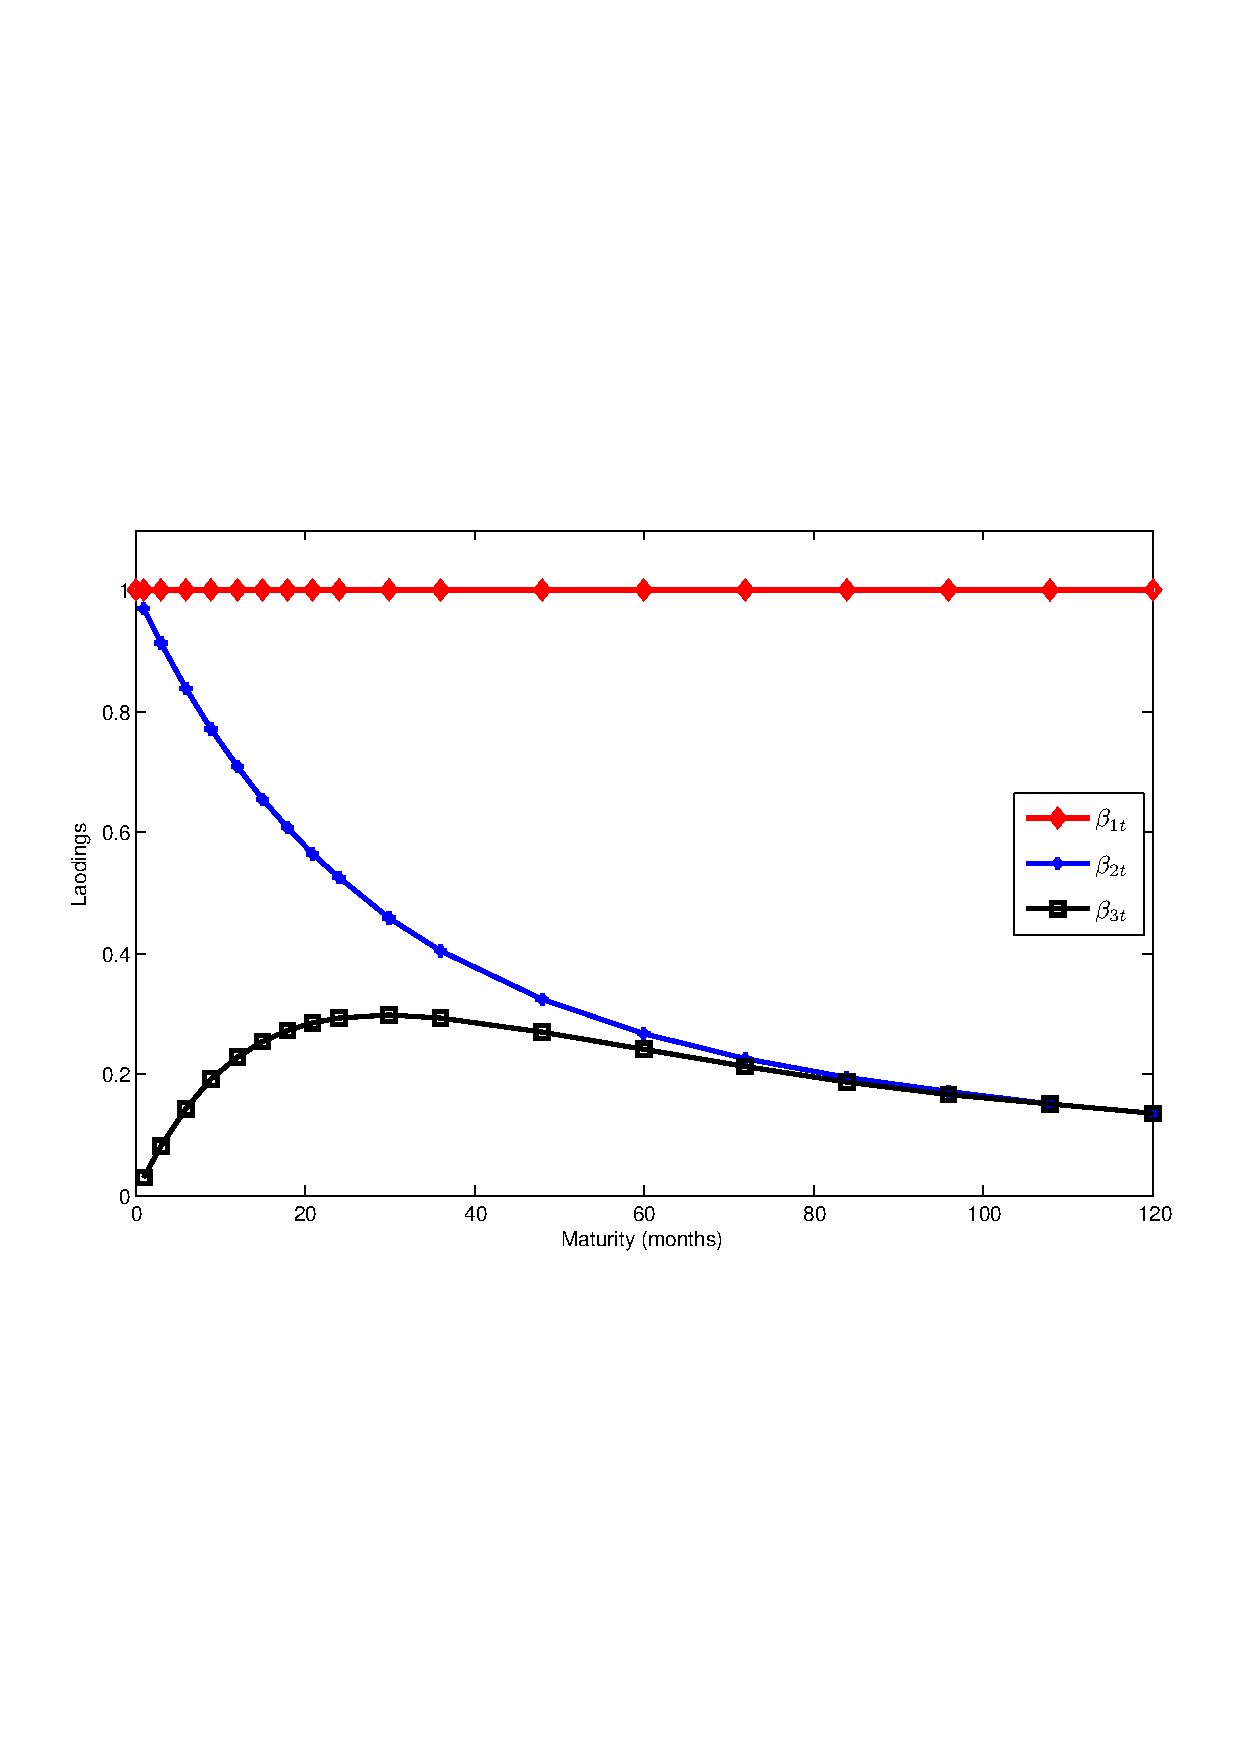
\includegraphics[width=15cm,height=8.5cm]{figures/tale_fig03}
    \caption{\dns 的因子载荷分析}
   \label{tale_fig03}
  \end{figure}

\subsection{影响因子的经济解释}{Economic Interpretation of DNS Model}\label{econ}

相比于其他\tsm{},\dns 中的因子所包含的经济意义更加明确。模型的因子载荷(Factor Loading)为
  \begin{align*}
    \bigg[ 1, \frac{1-e^{-\lambda_{t} \tau}} {\lambda_{t} \tau},
    \frac{1-e^{-\lambda_{t} \tau}} {\lambda_{t} \tau} - e^{-\lambda_{t} \tau} \bigg],
  \end{align*}
如图~\eqref{tale_fig03}~所示。三个隐含因子,$\bm{\beta}_t=(\beta_{1t},\beta_{2t},\beta_{3t})'$,很好的刻画了收益率曲线的长期、短期与中期的动态特征:
\begin{description}
  \item[水平因子] $\beta_{1t}$~的因子载荷为常数项~1~,即 \[\beta_{1t}=y_{t}(\infty)=\lim_{t\rightarrow \infty} \Big\{\beta_{1t}
        + \beta_{2t} \big[\frac{1-e^{-\lambda_{t} \tau}} {\lambda_{t} \tau} \big]
        + \beta_{3t}\big[\frac{1-e^{-\lambda_{t} \tau}} {\lambda_{t} \tau} - e^{-\lambda_{t} \tau} \big]\Big\},\]
        即~$\beta_{1t}$~是到期期限趋于无穷时~$y_t{\tau}$~的极限,在实际中,被看做是长期均衡条件下的利率水平,$\beta_{1t}$~ 的变动代表了整体债券市场的未来变动方向。这个因子受到经济系统基础层面的影响,如代表性消费者的投资风险厌恶程度的改变、社会结构尤其是人口年龄结构的波动等。
  \item[斜度因子] \dns 的第二个部分~$\beta_{2t}$~的载荷因子是到期期限~$\tau$~ 的指数递减函数,从~1~开始随着期限的增加而迅速衰减为~0~,这反映的是短期利率的变化情况,受到宏观政策冲击、长短期利差、金融市场噪声等影响。
  \item[曲度因子] 而~$\beta_{3t}$~的载荷因子是~$\Big[\frac{1-e^{-\lambda_{t} \tau}} {\lambda_{t} \tau} - e^{-\lambda_{t} \tau}\Big]$,一开始从~0~处逐渐递增,在中间部位达到最大值,然后随着到期期限的延长开始缓慢递减直至为~0。这表明~$\beta_{3t}$~主要对中期期限的收益率有较多的影响,而对长期及短期收益率部分没有影响,从而改变的是收益率曲线的曲度。
\end{description}
模型参数~$\bm{\beta}_t=(\beta_{1t},\beta_{2t},\beta_{3t})'$~的取值情况,决定了\ts 的动态特征,可以很好地刻画出不同收益率曲线的单调(monotonic)、驼峰(humped)以及~S~形状等多种形态,由模型拟合的形状与实际的利率曲线结构比较相符。同时,这三个动态因子也服从一个向量自回归过程(VAR):
  \begin{align}
    \bm{\beta}_t &= \bm{\mu} + \bm{\Phi}(L)\bm{\beta}_{t-1} + \bm{\eps}_t,
  \end{align}
    式中,$\bm{\beta}_t = \big[\beta_{1t}, \beta_{2t}, \beta_{3t}\big]'$, $\bm{\Phi}(L)$~ 为滞后运算因子(lag operation),且有~$\E_t[\bm{\eps}_t]=0$,$\E_t[\bm{\eps}_t \bm{\eps}_t']=\bm{\Omega}$,对于任何的非负值~$k$,$\E_t[\bm{\eps}_t \bm{\eps}_{t-k}']=\bm{0}$,即干扰项服从独立正态分布:$\bm{\eps}_t \sim \mathcal{N}(0,\bm{\Omega})$。

%\subsection{利率水平的变动与预测}
\subsection{模型估计与预测}
\dns 中的参数不在是常数项,而是一个服从向量自回归过程(VAR)的隐含因子(Latent Factors),可表示为状态空间方程(State Function),而到期收益率与影响因子之间的关系构成测量方程(Measurement Function),即
\begin{align}
\bm{y_t(\tau)} &= \mathcal{\bm{M}}(\bm{\tau}) \bm{\beta}_t  + \bm{\xi}_t, \\
\bm{\beta}_t &= \bm{\mu} + \bm{\Phi}(L)\bm{\beta}_{t-1} + \bm{\eps}_t,
\end{align}
%\end{subequaytions*}
式中,
\begin{align*}
\bm{y_t(\tau)} &=
  \begin{pmatrix}
    y_t(\tau_1) \\
    y_t(\tau_2) \\
    \vdots \\
    y_t(\tau_T) \\
  \end{pmatrix},\quad
  %%
  \mathcal{\bm{M}}(\bm{\tau}) =
  \begin{pmatrix}
    1 & \frac{1-e^{-\lambda_{t} \tau_1}} {\lambda_{t} \tau_1} & \frac{1-e^{-\lambda_{t} \tau_1}} {\lambda_{t} \tau_1} - e^{-\lambda_{t} \tau_1} \\
    1 & \frac{1-e^{-\lambda_{t} \tau_2}} {\lambda_{t} \tau_2} & \frac{1-e^{-\lambda_{t} \tau_2}} {\lambda_{t} \tau_2} - e^{-\lambda_{t} \tau_2} \\
\vdots    & \vdots &  \vdots\\
    1 & \frac{1-e^{-\lambda_{t} \tau_T}} {\lambda_{t} \tau_T} & \frac{1-e^{-\lambda_{t} \tau_T}} {\lambda_{t} \tau_T} - e^{-\lambda_{t} \tau_T} \\
  \end{pmatrix},\quad
  %%
   \bm{\beta}_t =
  \begin{pmatrix}
    \beta_{1t} \\
    \beta_{2t} \\
    \beta_{3t} \\
  \end{pmatrix},\\
  %%
 \bm{\xi}_t &=
    \begin{pmatrix}
    \xi_{t}(\tau_1) \\
    \xi_{t} (\tau_2)\\
    \vdots                  \\
    \xi_{t}(\tau_T) \\
  \end{pmatrix},\sim \mathcal{N}(0,\bm{\daleth}),\qquad
 \bm{\eps}_t =
    \begin{pmatrix}
    \varepsilon_{t}(\tau_1) \\
    \varepsilon_{t} (\tau_2)\\
    \vdots                  \\
    \varepsilon_{t}(\tau_T) \\
  \end{pmatrix},\sim \mathcal{N}(0,\bm{\Omega}).
  %%
\end{align*}
在状态空间表示的情况下,可以采用~Kalman~滤波构造样本函数,通过最大化似然函数对模型参数进行估计,并将参数估计值带入状态空间模型即可得到隐含变量~$\bm{\beta}_t$~的平滑值。

\dns 所展现的收益率曲线的动态变化具有持续性特征,如水平因子~$\beta_{1t}$~ 的高度自相关可以很好的刻画出收益率曲线变化的强持续性,而斜度因子$\beta_{2t}$~的低自相关性则可以代表长短期利差的低持续性。同时,收益率曲线的远端波动较为稳定,反映了整体经济系统的长期变化趋势。
\citeai{diebold2006forecasting}论证了\dns 所具有的一些特性,尤其是能够刻画出整个收益率曲线的动态特征,且在一阶向量自回归(VAR(1))的情况下,模型的参数只需经过两步法就能得到估计。同时,该模型在预测方向尤为突出,优于一般的模型如利率随机游走模型(Random Walk Model)、收益率自回归模型(AR(1))等模型,特别是\dns 在预测中长期收益率时均比其他模型有显著的提高。然而,对于为何\dns 能够对中长期零息票国债券收益率上有如此强劲的预测能力,\citeath{diebold2006forecasting}及其后的拓展模型并未给出明确的答案。
 
\section{人口年龄结构变动与利率期限结构}{Demographic Change}

一些人口经济学界和金融学家早已在上个世纪~90~年代开始关注\dsf 对金融市场特别是证券收益率的影响。下文将简要回顾已有的关文献资料,并指出所选取的代表\dsf 的指标变量的作用与意义。需要指出的是,目前关于\dsf 对\ts 的影响的研究尚处开始阶段,相关的理论与实证资料仍然欠缺。本文的研究目的之一就是希望能起到抛砖引玉的作用,有待后续的改善、提高。

%\subsection{人口年龄结构变动与债券价格和收益率}

人口年龄结构变动,尤其老龄化,是一个当今全球公认的亟待解决的问题,这在一些发达国家显得尤为突出。从个体家庭角度看,老龄化意味着每个生产性劳动力所需要供养的人口比例负担加大,相应的需要减少当前的消费水平并,并增加对未来不确定风险的投资,如增加储蓄、购买金融资产、养老保险等。而从社会总体看,这将导致生产性劳动力供给的下降、社会总体消费疲软、对未来不确定性的风险投资上升等。

然而,目前有关\dsf 与资产价格和收益率的相关关系的研究依然匮乏。正如\citeai{bakshi1994baby} 批评:
\begin{quotation}
  \dsf 能够通过各种方式影响经济动态。虽然已有经济学家着手研究\dsf 对社会总体消费、储蓄、劳动供给以及社会项目(social program)的影响,我们队\dsf 能否以及如何影响金融市场却知之甚少。
\end{quotation}

在少数的理论文献中,\citeai{bakshi1994baby}提出了一个引入\dsf 的代表性消费者资产定价模型(The Representative-Agent Pricing Model)。他们假设:典型的投资者的风险厌恶程度会随着年龄的增加而增加。由最优化投资决策条件可以推出表示代表性消费者对不同资本产品的投资需求的~Euler~ 方程:
 \begin{align}
   \E_t \bigg[\delta \cdot \frac{u_C(C_{t+\Delta t}, A_{t+\Delta t})}  {u_C(C_t,A_t)} \cdot \frac{P_{n,t+\Delta t}}{P_{n,t}} \bigg] =1.
 \end{align}
因此,通过影响金融市场上不同年龄阶段的投资者的生命周期投资策略(life-cycle portfolio investment strategies),\dsf 对金融市场的资产价格与回报率产生显著的影响。\citeai{abel2003effects}在一个世代交叠模型(OLG)的框架下分析了出生率变化与资产供给之间的关系,发现美国在二战后出现的婴儿潮人群相对于其他稳定的出生率的人群会导致资产价格上升,进而降低资产回报率。而\citeai{brooks2002asset} 则使用同样的模型,并利用模拟数据来分析\dsf 对风险贴水的影响。利用美国金融消费调查(Survey of Consumer Finances,SCF)中的横截面数据资料,\citeai{yoo1994age}发现\dsf 与短期国库券的实际利率之间有显著的负相关关系。在一篇总结性的文章里,\citeai{poterba2004impact}重新检验了\dsf 与国库券、长期政府债券及公司股票回报率之间的关系,得出了与\citeai{abel2003effects}不同的结论,即:各个年龄结构人口数量的变化与资本回报的相关关系十分微弱。

\citeai{geanakoplos2004demography}(以下简称~GMQ~模型)在一个封闭的经济模型基础上加入了\dsf{},提出了一个更加精细的世代交叠模型。GMQ~模型通过模拟美国婴儿出生率的动态特征,刻画了美国人口年龄结构变化的周期性变动(周期长度为~20~年)。他们根据美国在过去一个世纪内的人口年龄结构变化情况,将整个社会的人口总量按照年龄分为三个群体:(1)青年人群,由于收入不足以承担消费支出,在此阶段会通过资本市场进行借款;(2)中年群体,其收入迅速上升并超过支出,此时会倾向于将多余的收入进行投资(货币市场如银行机构,或者资本市场如购买证券);(3)退休群体,可以一次性的获得先前的所有投资款项以及相关收益,从而使用以前的储蓄收入以度晚年。该模型假设人口年龄结构在奇数期(odd)与偶数期(even)之间波动:
\begin{align}
  \Delta_t = (\Delta_t^y, \Delta_t^m, \Delta_t^r) =
      \left\{
    \begin{array}{cc}
      \Delta_1 = (N,n,N) & t=\text{奇数期} \\
      \Delta_2 = (n,N,n) & t=\text{偶数期} \\
    \end{array}
    \right.
\end{align}
式中,$\Delta_t^y$~表示青年人群的人口数量,$\Delta_t^m$~中年人群的人口数量,$\Delta_t^r$~表示退休人群的人口数量。由无套利机会条件(No-Arbitrage)可知
 \begin{align*}
  \frac{D+q_o^e}{q_e^e} & = \frac{1}{q_o} = 1+r_o \\
  \frac{D+q_e^e}{q_e^e} & = \frac{1}{q_e} = 1+r_e,
 \end{align*}
式中,$D$~表示股利分红,$q$~为股票价格,$q_o<q_e$($r_o>r_e$)意味着~$q_e^e<q_o^e$。而反映人口年龄结构动态特征的指标,$\frac{\Delta_t^m}{\Delta_t^y}$,对金融市场产生重要的影响:通过资本市场资金的借贷,不同年龄阶段的人口群体对金融产品的投资需求的变化决定了资本市场的均衡价格。在~GMQ~ 模型中,债券与股票被视为具有完全替代性的金融产品,\dsf 也决定了货币市场的长期均衡利率水平。基于有效市场假说关于资本市场具有信号指示的功能,\citeai{dellavigna2005attention} 探讨了\dsf 对即期与远期资本市场的影响,其研究结果显示,短期\dsf 对投资者的投资决策,进而对资产价格有重要影响。这种对不同金融市场的长期均衡价格与回报率的预测能力主要来自\dsf 具有稳定的可预测性。

以上文献资料主要关注\dsf 对金融市场价格的影响,而对于\dsf 与利率期限结构之间的关系,目前的研究尚处起步,仍未有一个统一的研究框架。其中较为成功的当属\citeai{favero2012demographics}在仿射利率期限结构模型(ATSM)中引入人口结构变量。在该模型中,
\begin{align*}
  y_t(\tau) &= -\frac{1}{\tau} \big( A_{\tau} + B_{\tau}' X_t + \Gamma_{\tau} \cdot MY_t(\tau) \big) + \eps_{t,t+1} \qquad \eps_{t,t+1} \sim \mathcal{N}(0,\sigma_2) \\
  r_t &= \delta_0 + \delta_1' X_t + \delta_2 MY_t  \\
  X_t &= \mu + \Phi X_{t-1} + \nu_t  \qquad \nu_{t,t+1} \sim i.i.d. \mathcal{N}(0,\Omega).
\end{align*}
式中,$MY_t$~为一个社会总人口中的中年人口与青年人口的总数比值。在该模型中,短期利率可表示为宏观状态变量~$X_t=[f_t^o,f_t^u]$~与当前社会人口变量~$MY_t$~ 的一个函数关系,而整个收益率曲线则与未来的\dsf 通过状态方程产生联系。\citeai{favero2012demographics}发现在仿射利率期限结构模型中引入反映人口年龄结构变化的变量能够很好的捕捉到长期均衡利率的持久性组成部分,从而比传统的利率期限期限结构模型能更好地解释长期利率的变化。
%\subsection{选取人口年龄变化的指标变量:$MY_t$}

根据\citeai{geanakoplos2004demography}及\citeai{favero2012demographics} 的研究,本文采用一个反映社会总人口中的中年人口(40-49)与青年人口(20-29)的总数比值,记作``$MY_t$''\nomenclature{$MY_t$}{一个社会总人口中的中年人口与青年人口的总数比值}。该比值变量能够很好的反映出货币市场长期均衡时的利率水平的变动状况。如图~\eqref{fig02}~ 和图~\eqref{fig01}~ 所示,$MY_t$~ (倒数)与不同期限的利率水平之间存在着强烈的协同运动(co-movement)的关系。值得注意的是,这种变动规律以大约一个代际(Generational Frequency)的时频出现交替轮换。$MY_t$~这一反映\dsf 的可预测指标能够较好的刻画出不同期限利率。%\footnote{这在\citeai{favero2012demographics}中也有类似的报告,但其未将长期均衡收益率与\dsf 之间的联动关系做进一步的解释。}

  \begin{figure}[!h]
    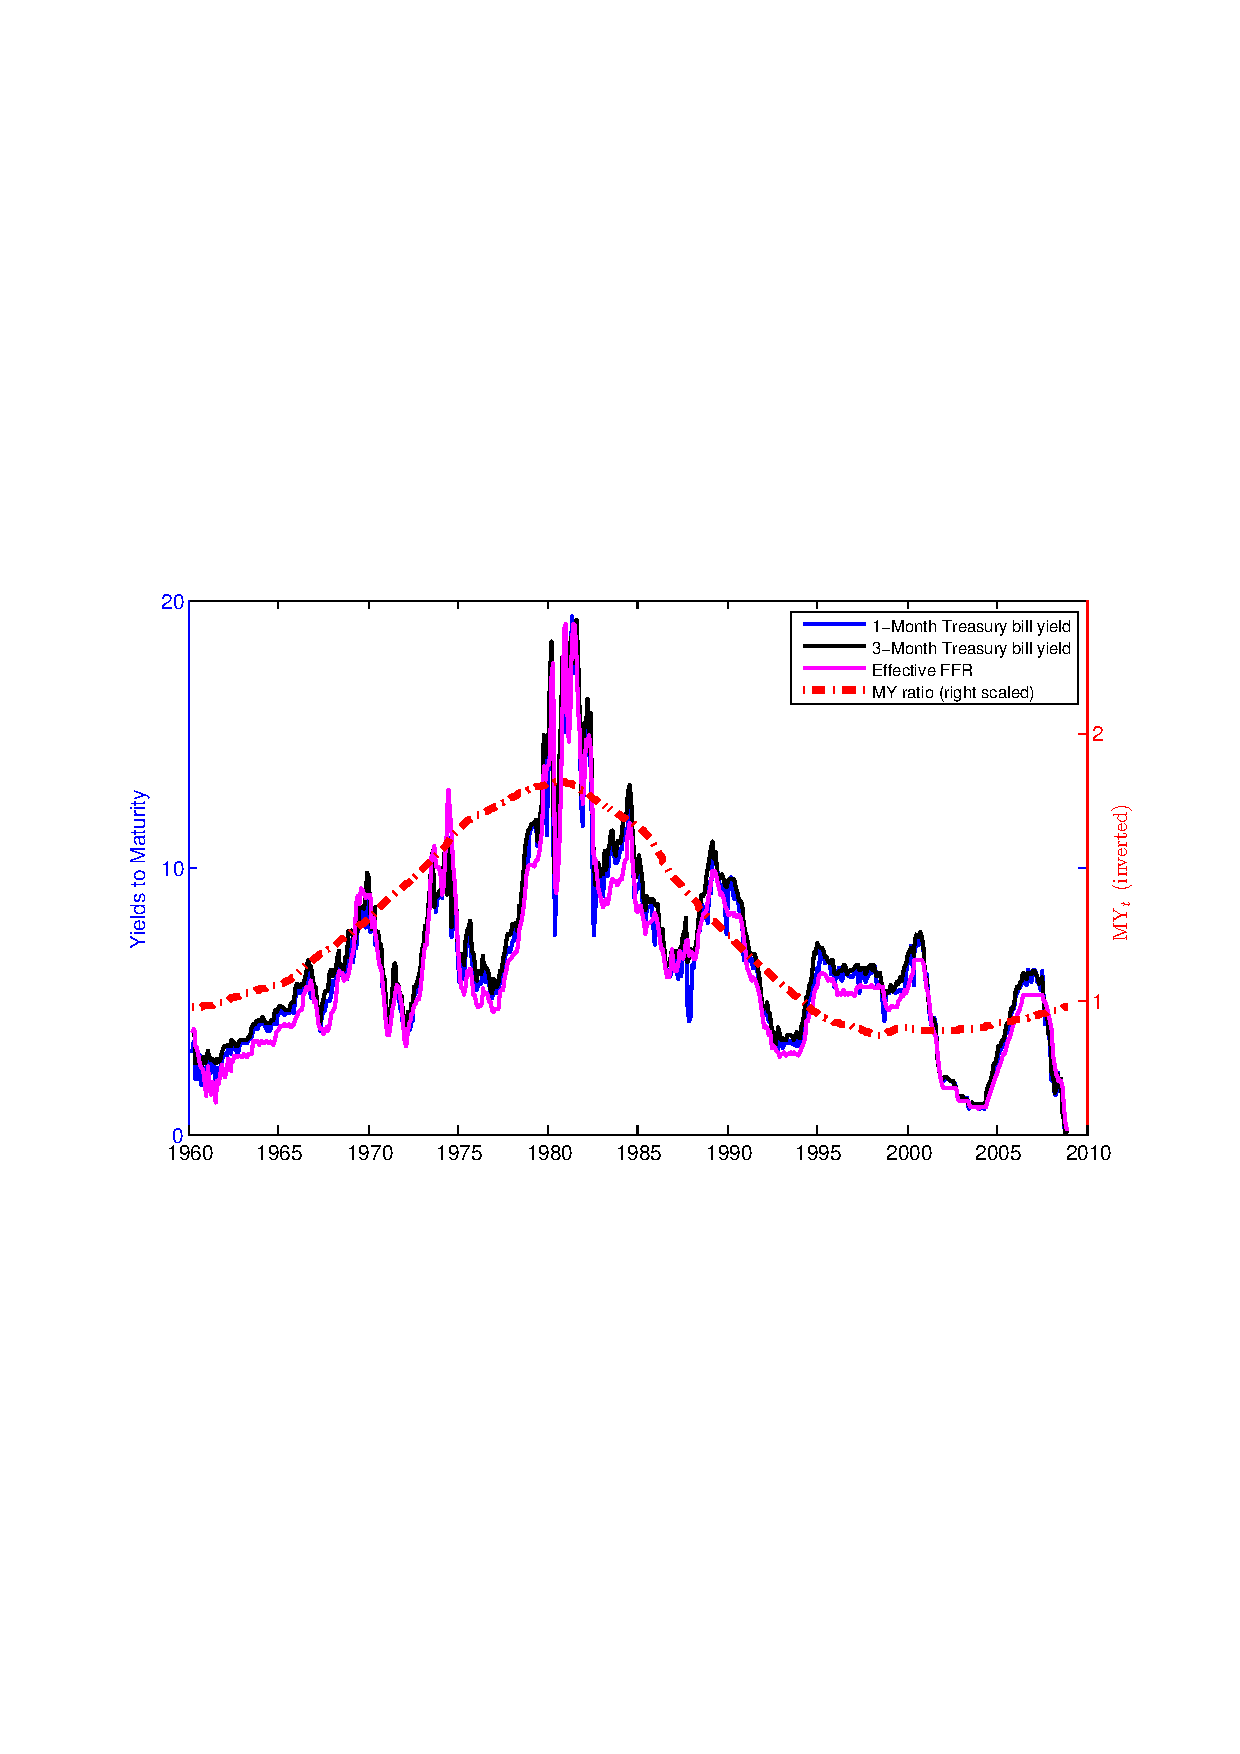
\includegraphics[width=15cm,height=8.5cm]{figures/fig02}
    \caption{美国短期利率与$MY_t$}    \label{fig02}
  \end{figure}

    \begin{figure}[!h]
    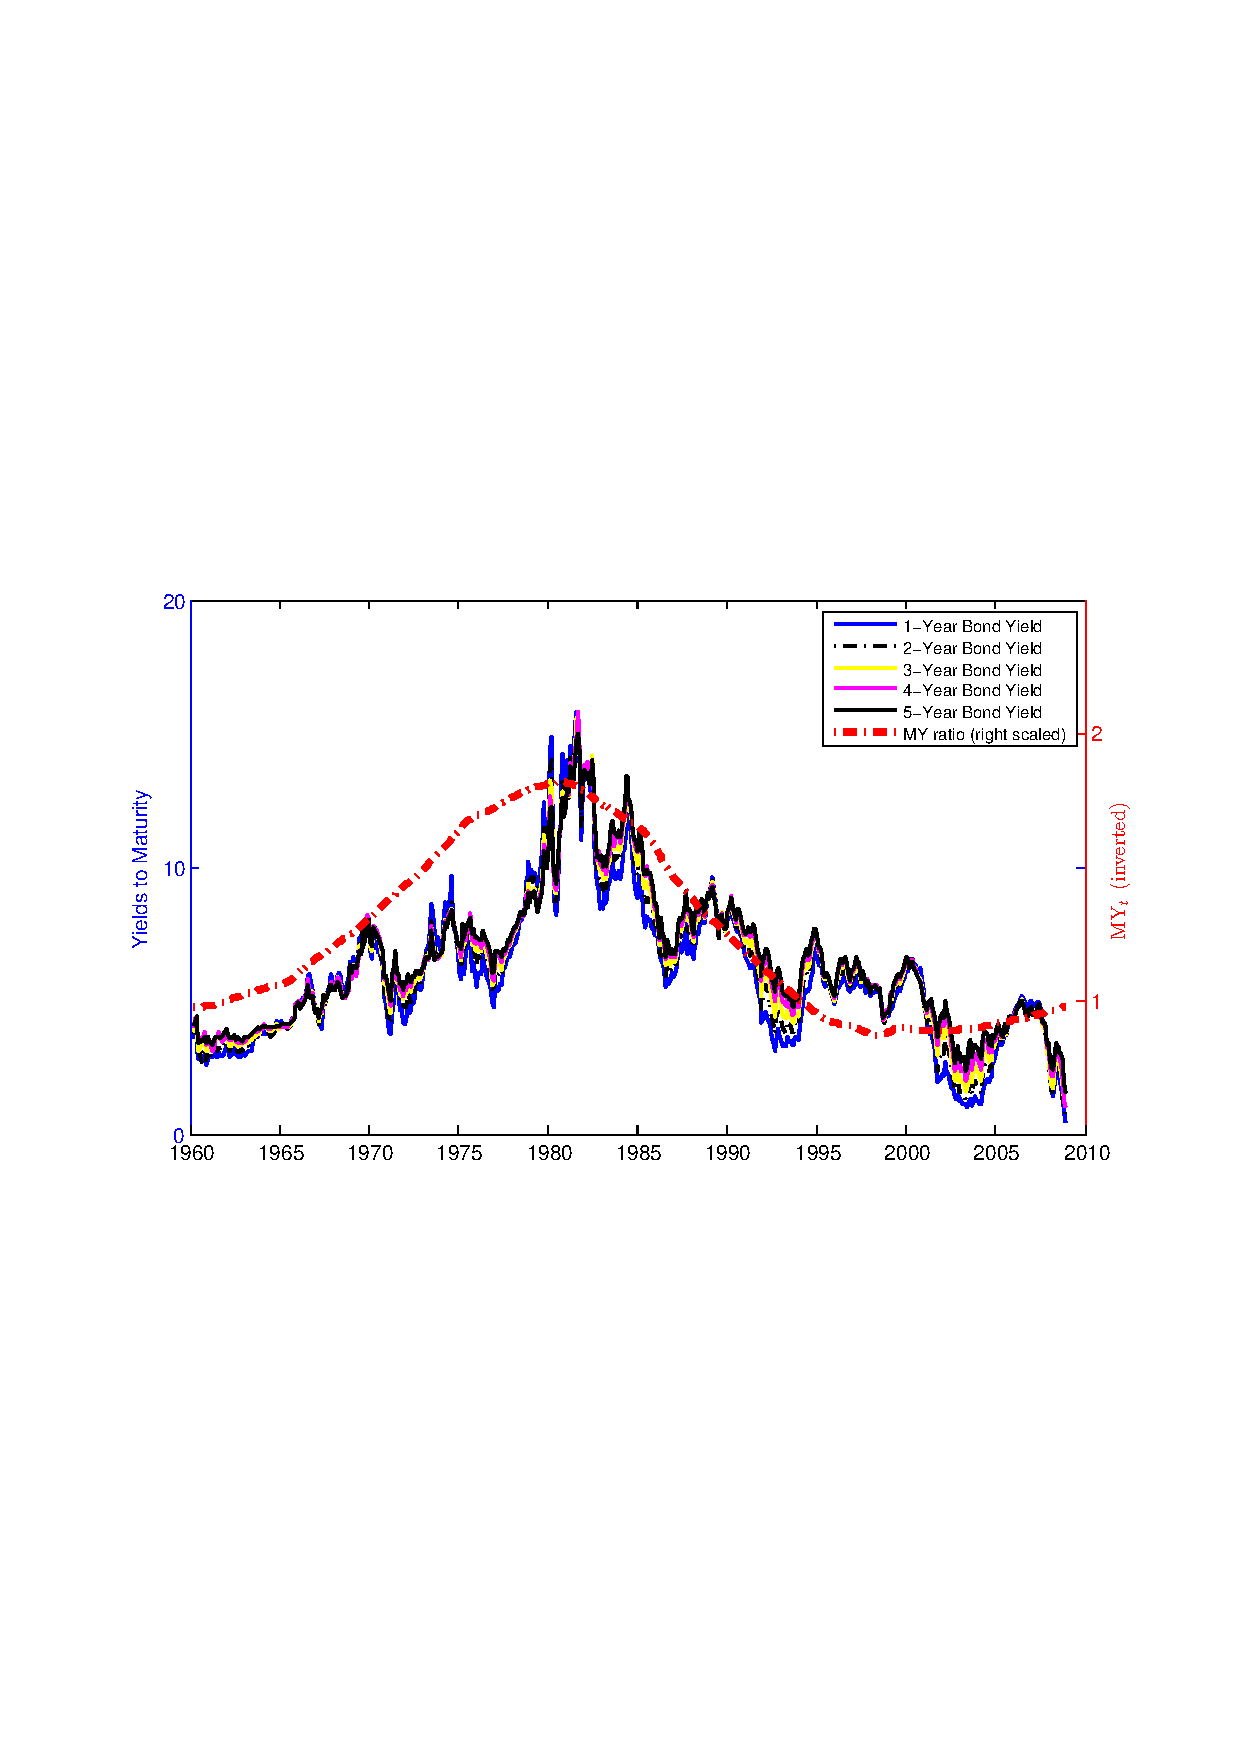
\includegraphics[width=15cm,height=8.5cm]{figures/fig01}
     \caption{中长期美国债券收益率与$MY_t$}    \label{fig01}
  \end{figure}

在直观上,当~$MY_t$~ 比较大(小),即在特定的时点上一个地区的中年群体(年轻群体)占总人口的比重较大,则这个中年群体由于收入大于支出从而推动了对储蓄(消费)的需求上升。在保证市场出清的条件下,利率则随之下降(上升)。GMQ~模型的实证研究也证实了理论研究的结论。即:股票实际回报率与~MY~存在显著的统计关系。\dsf 与不同期限利率的变动之间存在着紧密的关系,这也符合经济学的直觉推理。同时,在一定的时期内,\ds 具有相对可靠的预测性,可被视为一个外生变量,例如美国人口调查局(BoC)每五年都会进行一次人口预测项目(Population Projection)以提供未来的人口结构走势,该项目提供的报告具有一定的准确性。因此,建立一个由人口因素驱动的\tsm 不仅能够有助于增强\tsm 的理论解释能力,为理解影响长期均衡状态利率水平提供良好的理论支持,而在由于\dsf 的可预测性,将进一步提高对未来\tsm 变动的预测能力,从而为政策制定和市场投资提供有效的信息价值。

